\subsection{相对论重离子对撞中的双轻子产生}

如上节中提到的那样,双轻子是如今相对论重离子对撞物理中一个很重要的电磁探针。通过双轻子我们可以有手段对介质初期的演化进行研究。对于双轻子来说,其不变质量谱是一个重要的物理观测量,在 不同的质量区间有着不同的产生机制。同时也是唯一一种可以直接观测QCD介质中介质修正谱方程(In-medium spectral function of QCD medium)的手段。接下来会对不同质量区间的的双轻子产生机制进行简要的介绍。

对于整个的双轻子不变质量谱,根据其产生机制和物理目标不同我们主要将其分为三个不同的质量区间,分别是低质量区间(Low Mass Region, LMR, $M_{ee} < M_{\phi}$ ),中等质量区间(Intermediate Mass Region, IMR, $M_{\phi} < M_{ee} < M_{J/\psi}$)和高质量区间(High Mass Region, HMR, $M_{J/\psi} < M_{ee}$)。双轻子的不变质量越重,其产生于系统演化的越早期。

\begin{figure}[htb]
    \begin{center}
    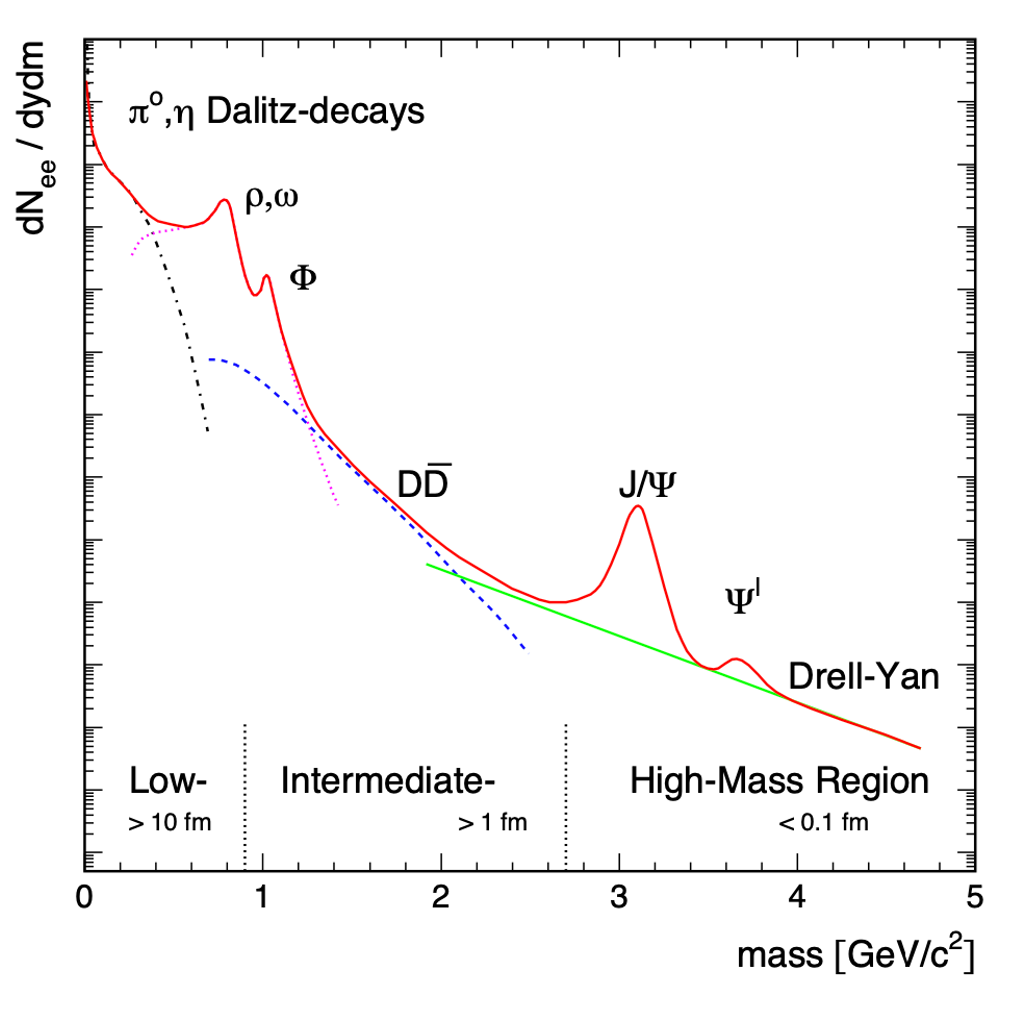
\includegraphics[width=0.8\textwidth,clip]{figures/Chapter1/DileptonSpectra.png}
    \end{center}
    \caption[双轻子不变质量谱示意图]{双轻子不变质量谱的质量区间划分和主要双轻子来源}
    \label{fig:DileptonSpectra}
\end{figure}

在高质量区间,双轻子主要来自于碰撞早期的部分子硬散射过程,例如Drell-Yan过程($q\bar{q} \rightarrow \gamma^*/Z \rightarrow l^{+}l^{-}$),重味夸克($c\bar{c}$, $b\bar{b}$)的半轻子衰变(semi-leptonic heavy flavor decays)以及重味夸克偶素的衰变($J/\psi, \psi(2S)$和$\Upsilon$)。

夸克偶素因为德拜屏蔽(Debye screening)在高温介质中解离成为夸克的过程被认为是夸克胶子等离子体存在的标志之一,因此夸克偶素在重离子对撞中的产额压低(Suppression)是重离子对撞物理中一个十分令人感兴趣的课题。在对离子-离子对撞中夸克偶素截面的核修正因子(Nuclear modification factor, $R_{AA}$)的测量观测到了这种产额压低的存在。同时在RHIC上也观测到到了在前向快度区间($1.2 < |y| < 2.2$)相比于中间快度区间($|\eta <0.35|$)有着更强的产额压低,这意味着除了色屏蔽以外可能有着其他的机制对夸克偶素的产额有着影响。目前常见的理论有夸克偶素的重结合(Recombination),冷核物质效应(Cold Nuclear Matter effect, CNM)等。

在中等质量区间,双轻子的主要来源是璨(charm)夸克和底(bottom)夸克的半轻子衰变以及夸克胶子等离子体的热辐射。以璨夸克为例,在初始硬过程中产生的背对背的$c$和$\bar{c}$各自独立地强子化为$D$和$\bar{D}$介子,这些介子再进行半轻子衰变生成轻子。在强子化的过程中,这些强子继承了初始的$c\bar{c}$夸克对的关联性并将其带到了最后两个半轻子衰变的组成的轻子对当中。但因为介质对c夸克的影响,轻子和轻子之间的关联性将会发生一定的改变,对最后的不变质量谱产生影响。需要注意的是,在中等质量区间这部分来源于粲夸克半轻子衰变的双轻子产额远高于来源于夸克胶子等离子体热辐射的双轻子产额,这使得想要在此质量区间抽取来源于夸克胶子等离子体的热辐射的双轻子产额变得十分困难。给实验上测量带来了巨大的挑战。

对于小质量区间来说,双轻子对的主要来源是各种强子的衰变。在诸多强子的质量谱当中,$\rho$的质量谱在介质当中的演化是我们最感兴趣的部分。因为$\rho$的寿命为大约1.3 fm/c,远小于夸克胶子等离子体的寿命(在RHIC最高能量下的“中心”碰撞中大约为 10 fm/c),其不变质量谱明显地受到与介质相互作用的影响而发生了改变。这个相互作用主要来源于 $\pi^+ + \pi^- \leftrightarrow \rho$ 道的强耦合。这个不变质量谱的改变和手征对称性恢复相关。当手征对称性恢复发生的时候,两个不同的手征多重态的质量(如$\rho(770)$和$a_1(1260)$)发生简并。在实验上测量$a_1(1260)$的质量谱是很困难的,所以我们可以通过测量$\rho(770)$来对手征对称性的恢复进行测量。尽管相对于$a_1(1260)$的测量相对来说容易一些,在双轻子测量中测量$\rho(770)$质量谱依旧十分困难。这是因为在低质量区间除了由$\rho(770)$衰变产生的双轻子对,还有大量的来源于其他介子例如$\pi^0, \eta, \eta^\prime, \omega, \phi$等介子的衰变的双轻子对。为了抽取$\rho(770)$的不变质量谱,其他介子的不变质量谱需要通过某种手段从总的不变质量谱中扣除。对于所有已知产额的介子,可以通过模拟的方式来得到其在不同能量不同对撞系统下的不变质量谱,这样就可以从总的不变质量谱中扣除这些已知产额的介子的谱,剩下的便是想要测量的强子的质量谱。因为这种将多种介子的不变质量谱的模拟混合的方式就像调制鸡尾酒的时候将多种基酒混合在一起,这个模拟的方法被称作“强子衰变模拟(hadronic cocktail)”,将会在双轻子分析一章中进行详细的讨论。

综上所述,通过双轻子的不变质量谱可以对丰富的物理目标进行测量,在过去的几十年中各个合作组在不同能量下对多种对撞系统进行了双轻子谱的测量,在接下来的一个小节中将对近些年来双轻子测量进行一个简单的回顾。